\documentclass[a4paper,10pt,twocolumn]{ltjarticle}
\usepackage{kaitoushu}

\pgfplotsset{
  myaxis/.style={
    axis lines=middle,
    xlabel={$x$}, ylabel={$y$},
    every axis x label/.style={at={(ticklabel* cs:1)},anchor=west},
    every axis y label/.style={at={(ticklabel* cs:1)},anchor=south},
    tick label style={font=\scriptsize},
    label style={font=\small},
    width=5.5cm, height=5cm,
    grid=none,
    samples=200,
  }
}

\begin{document}

\problemrange{5章：三角関数（255--336）}

%=============================================================
% Basic (p.56)
%=============================================================

\mondai{255}{次の三角形において，$\alpha$の三角比を求めよ．}
\kotae{
$\sin=\dfrac{\text{対辺}}{\text{斜辺}}$，$\cos=\dfrac{\text{隣辺}}{\text{斜辺}}$，$\tan=\dfrac{\text{対辺}}{\text{隣辺}}$

(1) 三辺 $2,\,1,\,\sqrt{3}$（斜辺2）

$\sin\alpha=\dfrac{1}{2}$，$\cos\alpha=\dfrac{\sqrt{3}}{2}$，$\tan\alpha=\dfrac{1}{\sqrt{3}}=\dfrac{\sqrt{3}}{3}$

(2) 三辺 $\sqrt{7},\,\sqrt{3},\,2$（$(\sqrt{3})^{2}+2^{2}=7$ より斜辺 $\sqrt{7}$）

$\sin\alpha=\dfrac{2}{\sqrt{7}}=\dfrac{2\sqrt{7}}{7}$，$\cos\alpha=\dfrac{\sqrt{3}}{\sqrt{7}}=\dfrac{\sqrt{21}}{7}$，$\tan\alpha=\dfrac{2}{\sqrt{3}}=\dfrac{2\sqrt{3}}{3}$

(3) 三辺 $12,\,13,\,5$（$5^{2}+12^{2}=169=13^{2}$ より斜辺13）

$\sin\alpha=\dfrac{12}{13}$，$\cos\alpha=\dfrac{5}{13}$，$\tan\alpha=\dfrac{12}{5}$
}

\mondai{256}{次の式の値を求めよ．}
\kotae{
加法定理を逆に使って1つにまとめる．

(1) $\sin60°\cos30°-\cos60°\sin30°=\sin(60°-30°)=\sin30°=\dfrac{1}{2}$

(2) $\cos30°\cos60°+\sin30°\sin60°=\cos(30°-60°)=\cos30°=\dfrac{\sqrt{3}}{2}$

(3) $\dfrac{\tan60°-\tan45°}{1+\tan60°\tan45°}=\tan(60°-45°)=\tan15°$

$=\dfrac{\sqrt{3}-1}{1+\sqrt{3}}=\dfrac{(\sqrt{3}-1)^{2}}{2}=2-\sqrt{3}$
}

\mondai{257}{三角関数表を用いて，次の三角比を求めよ．}
\kotae{
(1) $\sin6°\approx0.1045$\quad (2) $\cos33°\approx0.8387$\quad (3) $\tan84°\approx9.5144$
}

\mondai{258}{高さ634\,mのスカイツリーを見上げる角度が22°のとき，距離を求めよ．}
\kotae{
$\tan22°=\dfrac{634}{d}$，$d=\dfrac{634}{\tan22°}\approx\dfrac{634}{0.4040}\approx1569$\,m
}

\mondai{259}{次の三角比を $45°$ より小さい角の三角比で表せ．}
\kotae{
(1) $\sin81°=\cos9°$\quad (2) $\cos56°=\sin34°$\quad (3) $\tan77°=\dfrac{1}{\tan13°}$
}

\mondai{260}{次の式の値を求めよ．}
\kotae{
(1) $\sin45°\cos135°-\cos45°\sin135°=\sin(45°-135°)=\sin(-90°)=-1$

(2) $\dfrac{\tan45°-\tan150°}{1+\tan45°\tan150°}=\tan(45°-150°)$

$\tan150°=-\dfrac{1}{\sqrt{3}}$ より $=\dfrac{1+\frac{1}{\sqrt{3}}}{1-\frac{1}{\sqrt{3}}}=\dfrac{\sqrt{3}+1}{\sqrt{3}-1}=2+\sqrt{3}$

(3) $\cos120°\cos150°+\tan120°\sin150°+\sin120°\tan135°$

$=\left(-\dfrac{1}{2}\right)\!\left(-\dfrac{\sqrt{3}}{2}\right)+(-\sqrt{3})\cdot\dfrac{1}{2}+\dfrac{\sqrt{3}}{2}\cdot(-1)=\dfrac{\sqrt{3}}{4}-\dfrac{\sqrt{3}}{2}-\dfrac{\sqrt{3}}{2}=-\dfrac{3\sqrt{3}}{4}$
}

\mondai{261}{三角関数表を用いて，次の三角比を求めよ．}
\kotae{
$\sin(180°-\theta)=\sin\theta$，$\cos(180°-\theta)=-\cos\theta$，$\tan(180°-\theta)=-\tan\theta$

(1) $\sin100°=\sin80°\approx0.9848$

(2) $\cos176°=-\cos4°\approx-0.9976$

(3) $\tan111°=-\tan69°\approx-2.6051$
}

%=============================================================
% Check (p.57)
%=============================================================

\mondai{262}{次の問いに答えよ．}
\kotae{
$\sin^{2}\alpha+\cos^{2}\alpha=1$ で残りを求める．

(1) $\alpha$鋭角，$\sin\alpha=\dfrac{1}{4}$：$\cos\alpha=\dfrac{\sqrt{15}}{4}$，$\tan\alpha=\dfrac{1}{\sqrt{15}}=\dfrac{\sqrt{15}}{15}$

(2) $\alpha$鈍角，$\sin\alpha=\dfrac{1}{4}$：$\cos\alpha=-\dfrac{\sqrt{15}}{4}$，$\tan\alpha=-\dfrac{\sqrt{15}}{15}$

(3) $\alpha$鈍角，$\cos\alpha=-\dfrac{5}{6}$：$\sin\alpha=\dfrac{\sqrt{11}}{6}$，$\tan\alpha=-\dfrac{\sqrt{11}}{5}$
}

\mondai{263}{$\tan\alpha$から$\sin\alpha$，$\cos\alpha$を求めよ．}
\kotae{
$1+\tan^{2}\alpha=\dfrac{1}{\cos^{2}\alpha}$ を使う．

(1) $\alpha$鋭角，$\tan\alpha=\dfrac{1}{3}$

$\cos^{2}\alpha=\dfrac{9}{10}$，$\cos\alpha=\dfrac{3\sqrt{10}}{10}$，$\sin\alpha=\dfrac{\sqrt{10}}{10}$

(2) $\alpha$鈍角，$\tan\alpha=-2$

$\cos^{2}\alpha=\dfrac{1}{5}$，$\cos\alpha=-\dfrac{\sqrt{5}}{5}$，$\sin\alpha=\dfrac{2\sqrt{5}}{5}$
}

\mondai{264}{$\triangle$ABCにおいて，正弦定理を用いて求めよ．}
\kotae{
$\dfrac{a}{\sin A}=\dfrac{b}{\sin B}=\dfrac{c}{\sin C}=2R$

(1) $b=4$，$A=30°$，$B=45°$

$\dfrac{a}{\sin30°}=\dfrac{4}{\sin45°}$，$a=\dfrac{4\sin30°}{\sin45°}=\dfrac{2}{\frac{\sqrt{2}}{2}}=2\sqrt{2}$

(2) $b=2$，$c=\sqrt{3}$，$B=45°$

$\dfrac{2}{\sin45°}=\dfrac{\sqrt{3}}{\sin C}$，$\sin C=\dfrac{\sqrt{3}\cdot\frac{\sqrt{2}}{2}}{2}=\dfrac{\sqrt{6}}{4}$

(3) $c=5$，$A=45°$，$B=105°$

$C=30°$．$\dfrac{a}{\sin45°}=\dfrac{5}{\sin30°}=10$，$a=10\cdot\dfrac{\sqrt{2}}{2}=5\sqrt{2}$
}

\mondai{265}{1辺が$a$の正三角形の外接円の半径を求めよ．}
\kotae{
$2R=\dfrac{a}{\sin60°}=\dfrac{2a}{\sqrt{3}}$ → $R=\dfrac{\sqrt{3}\,a}{3}$
}

\mondai{266}{余弦定理を用いて辺の長さを求めよ．}
\kotae{
$a^{2}=b^{2}+c^{2}-2bc\cos A$

(1) $b=4$，$c=\sqrt{3}$，$A=30°$

$a^{2}=16+3-8\sqrt{3}\cdot\dfrac{\sqrt{3}}{2}=19-12=7$，$a=\sqrt{7}$

(2) $a=\sqrt{3}$，$c=\sqrt{6}$，$B=135°$

$b^{2}=3+6-2\sqrt{18}\cdot\left(-\dfrac{\sqrt{2}}{2}\right)=9+6=15$，$b=\sqrt{15}$

(3) $a=3\sqrt{3}$，$b=2$，$C=150°$

$c^{2}=27+4-12\sqrt{3}\cdot\left(-\dfrac{\sqrt{3}}{2}\right)=31+18=49$，$c=7$
}

\mondai{267}{$a=2$，$b=4$，$c=5$のとき$\cos A$，$\cos B$，$\cos C$を求めよ．}
\kotae{
$\cos A=\dfrac{b^{2}+c^{2}-a^{2}}{2bc}=\dfrac{16+25-4}{40}=\dfrac{37}{40}$

$\cos B=\dfrac{a^{2}+c^{2}-b^{2}}{2ac}=\dfrac{4+25-16}{20}=\dfrac{13}{20}$

$\cos C=\dfrac{a^{2}+b^{2}-c^{2}}{2ab}=\dfrac{4+16-25}{16}=-\dfrac{5}{16}$
}

\mondai{268}{$\triangle$ABCの面積を求めよ．}
\kotae{
$S=\dfrac{1}{2}bc\sin A$

(1) $b=5$，$c=7$，$A=45°$：$S=\dfrac{35}{2}\cdot\dfrac{\sqrt{2}}{2}=\dfrac{35\sqrt{2}}{4}$

(2) $a=2$，$b=3$，$C=150°$：$S=\dfrac{1}{2}\cdot2\cdot3\cdot\dfrac{1}{2}=\dfrac{3}{2}$
}

\mondai{269}{$a=7$，$B=30°$，面積9のとき$c$を求めよ．}
\kotae{
$9=\dfrac{1}{2}\cdot7\cdot c\cdot\sin30°=\dfrac{7c}{4}$ → $c=\dfrac{36}{7}$
}

\mondai{270}{$a=5$，$b=6$，$c=9$のとき．}
\kotae{
(1) $\cos C=\dfrac{25+36-81}{60}=-\dfrac{1}{3}$

(2) $\sin C=\sqrt{1-\dfrac{1}{9}}=\dfrac{2\sqrt{2}}{3}$

(3) $S=\dfrac{1}{2}\cdot5\cdot6\cdot\dfrac{2\sqrt{2}}{3}=10\sqrt{2}$
}

\mondai{271}{ヘロンの公式で面積を求めよ．}
\kotae{
$S=\sqrt{s(s-a)(s-b)(s-c)}$，$s=\dfrac{a+b+c}{2}$

(1) $a=5$，$b=7$，$c=8$：$s=10$

$S=\sqrt{10\cdot5\cdot3\cdot2}=\sqrt{300}=10\sqrt{3}$

(2) $a=2$，$b=3$，$c=4$：$s=\dfrac{9}{2}$

$S=\sqrt{\dfrac{9}{2}\cdot\dfrac{5}{2}\cdot\dfrac{3}{2}\cdot\dfrac{1}{2}}=\dfrac{3\sqrt{15}}{4}$
}

%=============================================================
% Check (p.58)
%=============================================================

\mondai{272}{次の三角形で$\alpha$の三角比を求めよ．}
\kotae{
(1) 三辺 $\sqrt{2},\,\sqrt{7},\,3$（斜辺3）

$\sin\alpha=\dfrac{\sqrt{2}}{3}$，$\cos\alpha=\dfrac{\sqrt{7}}{3}$，$\tan\alpha=\dfrac{\sqrt{2}}{\sqrt{7}}=\dfrac{\sqrt{14}}{7}$

(2) 三辺 $1,\,2,\,\sqrt{5}$（斜辺$\sqrt{5}$）

$\sin\alpha=\dfrac{2}{\sqrt{5}}=\dfrac{2\sqrt{5}}{5}$，$\cos\alpha=\dfrac{1}{\sqrt{5}}=\dfrac{\sqrt{5}}{5}$，$\tan\alpha=2$
}

\mondai{273}{図において，$\tan15°$の値を求めよ．}
\kotae{
加法定理：$\tan15°=\tan(45°-30°)=\dfrac{\tan45°-\tan30°}{1+\tan45°\tan30°}=\dfrac{1-\frac{1}{\sqrt{3}}}{1+\frac{1}{\sqrt{3}}}=\dfrac{\sqrt{3}-1}{\sqrt{3}+1}=2-\sqrt{3}$
}

\mondai{274}{傾斜角$34°$，距離815\,mのケーブルカーの標高差．}
\kotae{
$815\sin34°=815\times0.5592\approx456$\,m
}

\mondai{275}{次の式の値を求めよ．}
\kotae{
(1) $\sin60°\cos30°+\cos120°\sin150°+\sin135°\cos180°$

$=\dfrac{3}{4}-\dfrac{1}{4}-\dfrac{\sqrt{2}}{2}=\dfrac{1-\sqrt{2}}{2}$

(2) $\dfrac{\tan30°-\tan135°-\tan180°}{1+\tan120°\tan45°}$

$=\dfrac{\frac{1}{\sqrt{3}}+1-0}{1-\sqrt{3}}=\dfrac{\frac{\sqrt{3}+1}{\sqrt{3}}}{1-\sqrt{3}}=\dfrac{\sqrt{3}+1}{\sqrt{3}(1-\sqrt{3})}=-\dfrac{2\sqrt{3}+3}{3}$
}

\mondai{276}{$\alpha$鈍角，$\cos\alpha=-\dfrac{2}{5}$のとき．}
\kotae{
$\sin\alpha=\dfrac{\sqrt{21}}{5}$，$\tan\alpha=-\dfrac{\sqrt{21}}{2}$
}

\mondai{277}{$\alpha$鈍角，$\tan\alpha=-3$のとき．}
\kotae{
$\cos\alpha=-\dfrac{\sqrt{10}}{10}$，$\sin\alpha=\dfrac{3\sqrt{10}}{10}$
}

\mondai{278}{$\triangle$ABCの計算．}
\kotae{
(1) $a=\sqrt{6}$，$B=105°$，$C=30°$ → $A=45°$

$2R=\dfrac{\sqrt{6}}{\sin45°}=2\sqrt{3}$，$R=\sqrt{3}$，$c=2\sqrt{3}\sin30°=\sqrt{3}$

(2) $a=3$，$b=5$，$C=120°$

$c^{2}=9+25+15=49$，$c=7$，$S=\dfrac{15\sqrt{3}}{4}$

(3) $a=3$，$b=8$，$c=7$

$\cos B=\dfrac{9+49-64}{42}=-\dfrac{1}{7}$，$\sin B=\dfrac{4\sqrt{3}}{7}$，$S=6\sqrt{3}$
}

%=============================================================
% Basic (p.63) 一般角・弧度法・三角関数
%=============================================================

\mondai{285}{次の角を表す動径を図示せよ．}
\kotae{
$360°$で割った余りで位置を判定．

(1) $630°=360°+270°$ → $270°$の位置（$y$軸負方向）

(2) $-310°=50°$（第1象限）

(3) $490°=130°$（第2象限）

(4) $-1120°=-1120+4\times360=320°$（第4象限）

(5) $2000°=2000-5\times360=200°$（第3象限）
}

\mondai{286}{次の角は第何象限の角か．}
\kotae{
(1) $210°$：第3\quad (2) $400°=40°$：第1\quad (3) $-740°=340°$：第4

(4) $820°=100°$：第2\quad (5) $-635°=85°$：第1
}

\mondai{287}{次の三角関数の値を求めよ．}
\kotae{
(1) $\sin210°=-\sin30°=-\dfrac{1}{2}$

(2) $\cos570°=\cos210°=-\dfrac{\sqrt{3}}{2}$

(3) $\tan390°=\tan30°=\dfrac{\sqrt{3}}{3}$

(4) $\sin630°=\sin270°=-1$

(5) $\cos(-225°)=\cos225°=-\dfrac{\sqrt{2}}{2}$

(6) $\tan(-480°)=\tan240°=\sqrt{3}$
}

\mondai{288}{次の角を弧度法で表せ．}
\kotae{
(1) $135°=\dfrac{3\pi}{4}$\quad (2) $36°=\dfrac{\pi}{5}$\quad (3) $-10°=-\dfrac{\pi}{18}$

(4) $240°=\dfrac{4\pi}{3}$\quad (5) $-190°=-\dfrac{19\pi}{18}$
}

\mondai{289}{次の角を60分法で表せ．}
\kotae{
(1) $\dfrac{\pi}{3}=60°$\quad (2) $\dfrac{5\pi}{4}=225°$\quad (3) $-\dfrac{2\pi}{5}=-72°$

(4) $\dfrac{7\pi}{3}=420°$\quad (5) $-\dfrac{\pi}{9}=-20°$
}

\mondai{290}{次の三角関数の値を求めよ．}
\kotae{
(1) $\sin\dfrac{5\pi}{3}=-\sin\dfrac{\pi}{3}=-\dfrac{\sqrt{3}}{2}$

(2) $\cos\dfrac{5\pi}{4}=-\cos\dfrac{\pi}{4}=-\dfrac{\sqrt{2}}{2}$

(3) $\tan\dfrac{\pi}{6}=\dfrac{\sqrt{3}}{3}$
}

\mondai{291}{弧の長さと扇形の面積を求めよ．}
\kotae{
$l=r\theta$，$S=\dfrac{1}{2}r^{2}\theta$

(1) 半径4，中心角$\dfrac{\pi}{6}$：$l=\dfrac{2\pi}{3}$，$S=\dfrac{4\pi}{3}$

(2) 半径3，弧$2\pi$：$\theta=\dfrac{2\pi}{3}$，$S=3\pi$
}

\mondai{292}{次の等式を証明せよ．}
\kotae{
(1) $\tan\theta+\dfrac{1}{\tan\theta}=\dfrac{\sin^{2}\theta+\cos^{2}\theta}{\sin\theta\cos\theta}=\dfrac{1}{\sin\theta\cos\theta}$ \qed

(2) $\dfrac{1}{1-\cos\theta}+\dfrac{1}{1+\cos\theta}=\dfrac{2}{1-\cos^{2}\theta}=\dfrac{2}{\sin^{2}\theta}$ \qed
}

\mondai{293}{象限と1つの三角関数の値から残りを求めよ．}
\kotae{
(1) 第3象限，$\sin\theta=-\dfrac{4}{5}$

$\cos\theta=-\dfrac{3}{5}$，$\tan\theta=\dfrac{4}{3}$

(2) 第4象限，$\cos\theta=\dfrac{1}{3}$

$\sin\theta=-\dfrac{2\sqrt{2}}{3}$，$\tan\theta=-2\sqrt{2}$

(3) 第3象限，$\tan\theta=3$

$\cos\theta=-\dfrac{\sqrt{10}}{10}$，$\sin\theta=-\dfrac{3\sqrt{10}}{10}$
}

\mondai{294}{次の式を簡単にせよ．}
\kotae{
(1) $\cos\theta\sin\!\left(\dfrac{\pi}{2}-\theta\right)+\sin\theta\cos\!\left(\dfrac{\pi}{2}-\theta\right)=\cos^{2}\theta+\sin^{2}\theta=1$

(2) $\sin\!\left(\dfrac{\pi}{2}-\theta\right)-\sin(\pi+\theta)+\cos\!\left(\dfrac{\pi}{2}+\theta\right)+\cos(\pi-\theta)$

$=\cos\theta+\sin\theta-\sin\theta-\cos\theta=0$

(3) $\tan(\pi+\theta)\sin\!\left(\dfrac{\pi}{2}+\theta\right)+\cos(\pi-\theta)\tan(\pi-\theta)$

$=\tan\theta\cos\theta+(-\cos\theta)(-\tan\theta)=\sin\theta+\sin\theta=2\sin\theta$
}

\mondai{295}{次の関数の周期を求め，グラフをかけ．}
\kotae{
(1) $y=\sin\!\left(x-\dfrac{\pi}{2}\right)=-\cos x$\quad 周期$2\pi$

\begin{tikzpicture}
\begin{axis}[myaxis, xmin=-0.5,xmax=7,ymin=-1.5,ymax=1.5,
  xtick={1.5708,3.1416,4.7124,6.2832},
  xticklabels={$\frac{\pi}{2}$,$\pi$,$\frac{3\pi}{2}$,$2\pi$}]
\addplot[thick,blue]{sin(deg(x-1.5708))};
\end{axis}
\end{tikzpicture}

(2) $y=\cos\!\left(x+\dfrac{\pi}{4}\right)$\quad 周期$2\pi$

\begin{tikzpicture}
\begin{axis}[myaxis, xmin=-0.5,xmax=7,ymin=-1.5,ymax=1.5,
  xtick={1.5708,3.1416,4.7124,6.2832},
  xticklabels={$\frac{\pi}{2}$,$\pi$,$\frac{3\pi}{2}$,$2\pi$}]
\addplot[thick,blue]{cos(deg(x+0.7854))};
\end{axis}
\end{tikzpicture}
}

\mondai{296}{次の関数の周期を求め，グラフをかけ．}
\kotae{
(1) $y=2\cos x$\quad 周期$2\pi$，振幅$2$

\begin{tikzpicture}
\begin{axis}[myaxis, xmin=-0.5,xmax=7,ymin=-2.5,ymax=2.5,
  xtick={1.5708,3.1416,4.7124,6.2832},
  xticklabels={$\frac{\pi}{2}$,$\pi$,$\frac{3\pi}{2}$,$2\pi$}]
\addplot[thick,blue]{2*cos(deg(x))};
\end{axis}
\end{tikzpicture}

(2) $y=-\dfrac{1}{2}\sin x$\quad 周期$2\pi$，振幅$\dfrac{1}{2}$

\begin{tikzpicture}
\begin{axis}[myaxis, xmin=-0.5,xmax=7,ymin=-1,ymax=1,
  xtick={1.5708,3.1416,4.7124,6.2832},
  xticklabels={$\frac{\pi}{2}$,$\pi$,$\frac{3\pi}{2}$,$2\pi$}]
\addplot[thick,blue]{-0.5*sin(deg(x))};
\end{axis}
\end{tikzpicture}
}

\mondai{297}{次の関数の周期を求め，グラフをかけ．}
\kotae{
$y=\sin(kx)$ の周期は $\dfrac{2\pi}{|k|}$．

(1) $y=\cos 2x$\quad 周期$\pi$

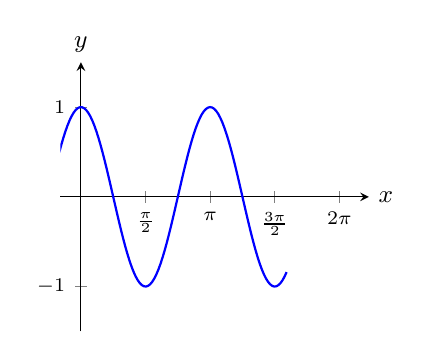
\begin{tikzpicture}
\begin{axis}[myaxis, xmin=-0.5,xmax=7,ymin=-1.5,ymax=1.5,
  xtick={1.5708,3.1416,4.7124,6.2832},
  xticklabels={$\frac{\pi}{2}$,$\pi$,$\frac{3\pi}{2}$,$2\pi$}]
\addplot[thick,blue]{cos(deg(2*x))};
\end{axis}
\end{tikzpicture}

(2) $y=\sin\dfrac{x}{3}$\quad 周期$6\pi$

\begin{tikzpicture}
\begin{axis}[myaxis, xmin=-0.5,xmax=20,ymin=-1.5,ymax=1.5,
  xtick={3.1416,6.2832,9.4248,12.5664,15.708,18.8496},
  xticklabels={$\pi$,$2\pi$,$3\pi$,$4\pi$,$5\pi$,$6\pi$},
  width=6.5cm]
\addplot[thick,blue]{sin(deg(x/3))};
\end{axis}
\end{tikzpicture}
}

\mondai{298}{$0\leqq x<2\pi$ で方程式・不等式を解け．}
\kotae{
(1) $\sin x=\dfrac{\sqrt{2}}{2}$ → $x=\dfrac{\pi}{4},\;\dfrac{3\pi}{4}$

(2) $\cos x=\dfrac{1}{2}$ → $x=\dfrac{\pi}{3},\;\dfrac{5\pi}{3}$

(3) $\sin x\geqq\dfrac{\sqrt{3}}{2}$ → $\dfrac{\pi}{3}\leqq x\leqq\dfrac{2\pi}{3}$

(4) $\cos x<-\dfrac{\sqrt{2}}{2}$ → $\dfrac{3\pi}{4}<x<\dfrac{5\pi}{4}$
}

\mondai{299}{$0\leqq x<2\pi$ で方程式を解け．}
\kotae{
(1) $\tan x=0$ → $x=0,\;\pi$

(2) $\tan x=-1$ → $x=\dfrac{3\pi}{4},\;\dfrac{7\pi}{4}$
}

%=============================================================
% Check (p.65)
%=============================================================

\mondai{300}{次の角を弧度法で表せ．}
\kotae{
(1) $40°=\dfrac{2\pi}{9}$\quad (2) $50°=\dfrac{5\pi}{18}$\quad (3) $-18°=-\dfrac{\pi}{10}$\quad (4) $-210°=-\dfrac{7\pi}{6}$
}

\mondai{301}{次の角を60分法で表せ．}
\kotae{
(1) $\dfrac{7\pi}{6}=210°$\quad (2) $\dfrac{5\pi}{3}=300°$\quad (3) $-\dfrac{4\pi}{9}=-80°$\quad (4) $-\dfrac{11\pi}{4}=-495°$
}

\mondai{302}{半径6，中心角$\dfrac{5\pi}{6}$の扇形の弧の長さ$l$と面積$S$を求めよ．}
\kotae{
$l=6\cdot\dfrac{5\pi}{6}=5\pi$，$S=\dfrac{1}{2}\cdot36\cdot\dfrac{5\pi}{6}=15\pi$
}

\mondai{303}{次の三角関数の値を求めよ．}
\kotae{
(1) $\sin\dfrac{11\pi}{6}=\sin\!\left(2\pi-\dfrac{\pi}{6}\right)=-\sin\dfrac{\pi}{6}=-\dfrac{1}{2}$

(2) $\cos\!\left(-\dfrac{5\pi}{4}\right)=\cos\dfrac{5\pi}{4}=-\cos\dfrac{\pi}{4}=-\dfrac{\sqrt{2}}{2}$

(3) $\tan\!\left(-\dfrac{5\pi}{3}\right)=\tan\!\left(-\dfrac{5\pi}{3}+2\pi\right)=\tan\dfrac{\pi}{3}=\sqrt{3}$
}

\mondai{304}{$\theta$が第2象限で$\sin\theta=\dfrac{2}{3}$のとき，$\cos\theta$，$\tan\theta$を求めよ．}
\kotae{
$\cos^{2}\theta=1-\dfrac{4}{9}=\dfrac{5}{9}$．第2象限で$\cos<0$：$\cos\theta=-\dfrac{\sqrt{5}}{3}$

$\tan\theta=\dfrac{2/3}{-\sqrt{5}/3}=-\dfrac{2}{\sqrt{5}}=-\dfrac{2\sqrt{5}}{5}$
}

\mondai{305}{次の式を簡単にせよ．}
\kotae{
(1) $\sin(\pi+\theta)\cos(2\pi-\theta)+\sin\!\left(\dfrac{\pi}{2}+\theta\right)\cos(\pi-\theta)$

$=(-\sin\theta)(\cos\theta)+(\cos\theta)(-\cos\theta)=-\sin\theta\cos\theta-\cos^{2}\theta$

$=-\cos\theta(\sin\theta+\cos\theta)$

(2) $\dfrac{\sin(\pi-\theta)}{\cos\!\left(\frac{\pi}{2}+\theta\right)}-\dfrac{\tan(\pi+\theta)\cos(\pi+\theta)}{\sin\!\left(\frac{3\pi}{2}-\theta\right)}$

$=\dfrac{\sin\theta}{-\sin\theta}-\dfrac{\tan\theta\cdot(-\cos\theta)}{-\cos\theta}=-1-\tan\theta$
}

\mondai{306}{次の等式を証明せよ．}
\kotae{
(1) $\dfrac{1}{1+\sin\theta}+\dfrac{1}{1-\sin\theta}=\dfrac{2}{\cos^{2}\theta}$

左辺$=\dfrac{(1-\sin\theta)+(1+\sin\theta)}{1-\sin^{2}\theta}=\dfrac{2}{\cos^{2}\theta}=$右辺 \qed

(2) $\sin^{4}\theta-\cos^{4}\theta=\sin^{2}\theta-\cos^{2}\theta$

左辺$=(\sin^{2}\theta+\cos^{2}\theta)(\sin^{2}\theta-\cos^{2}\theta)=1\cdot(\sin^{2}\theta-\cos^{2}\theta)=$右辺 \qed
}

\mondai{307}{次の関数の周期とグラフをかけ．}
\kotae{
(1) $y=3\sin x$\quad 周期$2\pi$，振幅$3$

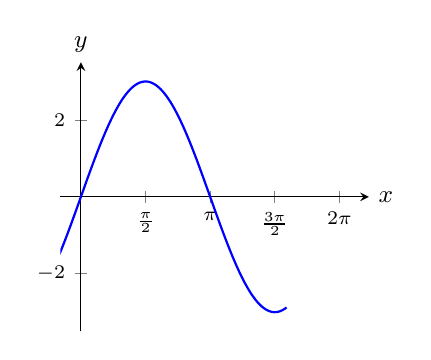
\begin{tikzpicture}
\begin{axis}[myaxis, xmin=-0.5,xmax=7,ymin=-3.5,ymax=3.5,
  xtick={1.5708,3.1416,4.7124,6.2832},
  xticklabels={$\frac{\pi}{2}$,$\pi$,$\frac{3\pi}{2}$,$2\pi$}]
\addplot[thick,blue]{3*sin(deg(x))};
\end{axis}
\end{tikzpicture}

(2) $y=\sin 3x$\quad 周期$\dfrac{2\pi}{3}$

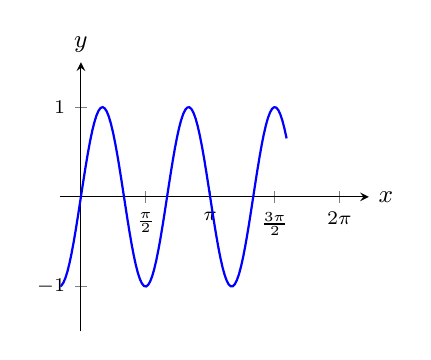
\begin{tikzpicture}
\begin{axis}[myaxis, xmin=-0.5,xmax=7,ymin=-1.5,ymax=1.5,
  xtick={1.5708,3.1416,4.7124,6.2832},
  xticklabels={$\frac{\pi}{2}$,$\pi$,$\frac{3\pi}{2}$,$2\pi$}]
\addplot[thick,blue]{sin(deg(3*x))};
\end{axis}
\end{tikzpicture}

(3) $y=\cos\!\left(x-\dfrac{\pi}{3}\right)$\quad 周期$2\pi$

\begin{tikzpicture}
\begin{axis}[myaxis, xmin=-0.5,xmax=7,ymin=-1.5,ymax=1.5,
  xtick={1.5708,3.1416,4.7124,6.2832},
  xticklabels={$\frac{\pi}{2}$,$\pi$,$\frac{3\pi}{2}$,$2\pi$}]
\addplot[thick,blue]{cos(deg(x-1.0472))};
\end{axis}
\end{tikzpicture}
}

\mondai{308}{$0\leqq x<2\pi$ で次を解け．}
\kotae{
(1) $2\cos x+\sqrt{3}=0$ → $\cos x=-\dfrac{\sqrt{3}}{2}$

$x=\dfrac{5\pi}{6},\;\dfrac{7\pi}{6}$

(2) $\tan x+1\geqq0$ → $\tan x\geqq-1$

$\tan x=-1$ となるのは $x=\dfrac{3\pi}{4},\;\dfrac{7\pi}{4}$

$\therefore 0\leqq x<\dfrac{\pi}{2}$ または $\dfrac{3\pi}{4}\leqq x<\dfrac{3\pi}{2}$ または $\dfrac{7\pi}{4}\leqq x<2\pi$

（$\tan$ の定義域に注意：$x\neq\dfrac{\pi}{2},\;\dfrac{3\pi}{2}$）
}

%=============================================================
% Basic (p.69) 加法定理・倍角・合成
%=============================================================

\mondai{318}{次の値を求めよ．}
\kotae{
加法定理：$\sin(\alpha\pm\beta)=\sin\alpha\cos\beta\pm\cos\alpha\sin\beta$，$\cos(\alpha\pm\beta)=\cos\alpha\cos\beta\mp\sin\alpha\sin\beta$

(1) $\sin75°=\sin(45°+30°)=\dfrac{\sqrt{2}}{2}\cdot\dfrac{\sqrt{3}}{2}+\dfrac{\sqrt{2}}{2}\cdot\dfrac{1}{2}=\dfrac{\sqrt{6}+\sqrt{2}}{4}$

(2) $\cos15°=\cos(45°-30°)=\dfrac{\sqrt{2}}{2}\cdot\dfrac{\sqrt{3}}{2}+\dfrac{\sqrt{2}}{2}\cdot\dfrac{1}{2}=\dfrac{\sqrt{6}+\sqrt{2}}{4}$

(3) $\tan\dfrac{5\pi}{12}=\tan(75°)=\tan(45°+30°)=\dfrac{1+\frac{1}{\sqrt{3}}}{1-\frac{1}{\sqrt{3}}}=\dfrac{\sqrt{3}+1}{\sqrt{3}-1}=2+\sqrt{3}$
}

\mondai{319}{$\alpha$が第2象限で$\sin\alpha=\dfrac{4}{5}$，$\beta$が第1象限で$\cos\beta=\dfrac{5}{13}$のとき，$\sin(\alpha+\beta)$，$\cos(\alpha-\beta)$ を求めよ．}
\kotae{
$\cos\alpha=-\dfrac{3}{5}$（第2象限），$\sin\beta=\dfrac{12}{13}$（第1象限）

$\sin(\alpha+\beta)=\dfrac{4}{5}\cdot\dfrac{5}{13}+\left(-\dfrac{3}{5}\right)\cdot\dfrac{12}{13}=\dfrac{20}{65}-\dfrac{36}{65}=-\dfrac{16}{65}$

$\cos(\alpha-\beta)=\left(-\dfrac{3}{5}\right)\cdot\dfrac{5}{13}+\dfrac{4}{5}\cdot\dfrac{12}{13}=-\dfrac{15}{65}+\dfrac{48}{65}=\dfrac{33}{65}$
}

\mondai{320}{$\sin\alpha=\dfrac{1}{\sqrt{5}}$，$\sin\beta=\dfrac{1}{\sqrt{10}}$（$\alpha,\beta$は鋭角）のとき，$\alpha+\beta$を求めよ．}
\kotae{
$\cos\alpha=\dfrac{2}{\sqrt{5}}$，$\cos\beta=\dfrac{3}{\sqrt{10}}$

$\sin(\alpha+\beta)=\dfrac{1}{\sqrt{5}}\cdot\dfrac{3}{\sqrt{10}}+\dfrac{2}{\sqrt{5}}\cdot\dfrac{1}{\sqrt{10}}=\dfrac{3}{\sqrt{50}}+\dfrac{2}{\sqrt{50}}=\dfrac{5}{5\sqrt{2}}=\dfrac{1}{\sqrt{2}}$

$\alpha+\beta$ は鋭角の和なので $0<\alpha+\beta<\pi$．$\sin(\alpha+\beta)=\dfrac{\sqrt{2}}{2}$ より

$\alpha+\beta=\dfrac{\pi}{4}$ または $\dfrac{3\pi}{4}$

$\cos(\alpha+\beta)=\dfrac{2}{\sqrt{5}}\cdot\dfrac{3}{\sqrt{10}}-\dfrac{1}{\sqrt{5}}\cdot\dfrac{1}{\sqrt{10}}=\dfrac{5}{\sqrt{50}}=\dfrac{1}{\sqrt{2}}>0$ より

$\alpha+\beta=\dfrac{\pi}{4}$
}

\mondai{321}{2倍角の公式を用いて，次の値を求めよ．}
\kotae{
$\sin2\alpha=2\sin\alpha\cos\alpha$，$\cos2\alpha=1-2\sin^{2}\alpha=2\cos^{2}\alpha-1$

(1) $\sin\dfrac{\pi}{8}$

$\cos\dfrac{\pi}{4}=1-2\sin^{2}\dfrac{\pi}{8}$，$\dfrac{\sqrt{2}}{2}=1-2\sin^{2}\dfrac{\pi}{8}$

$\sin^{2}\dfrac{\pi}{8}=\dfrac{2-\sqrt{2}}{4}$，$\sin\dfrac{\pi}{8}=\dfrac{\sqrt{2-\sqrt{2}}}{2}$

(2) $\cos\dfrac{\pi}{8}$

$\cos\dfrac{\pi}{4}=2\cos^{2}\dfrac{\pi}{8}-1$，$\cos^{2}\dfrac{\pi}{8}=\dfrac{2+\sqrt{2}}{4}$

$\cos\dfrac{\pi}{8}=\dfrac{\sqrt{2+\sqrt{2}}}{2}$
}

\mondai{322}{$\theta$が第3象限で$\cos\theta=-\dfrac{3}{4}$のとき，$\sin2\theta$，$\cos2\theta$，$\tan2\theta$を求めよ．}
\kotae{
$\sin^{2}\theta=1-\dfrac{9}{16}=\dfrac{7}{16}$．第3象限で$\sin<0$：$\sin\theta=-\dfrac{\sqrt{7}}{4}$

$\sin2\theta=2\cdot\left(-\dfrac{\sqrt{7}}{4}\right)\!\left(-\dfrac{3}{4}\right)=\dfrac{3\sqrt{7}}{8}$

$\cos2\theta=2\cos^{2}\theta-1=2\cdot\dfrac{9}{16}-1=\dfrac{1}{8}$

$\tan2\theta=\dfrac{\sin2\theta}{\cos2\theta}=\dfrac{3\sqrt{7}/8}{1/8}=3\sqrt{7}$
}

\mondai{323}{三角関数の合成を行え．}
\kotae{
$a\sin\theta+b\cos\theta=\sqrt{a^{2}+b^{2}}\sin(\theta+\varphi)$（$\tan\varphi=\dfrac{b}{a}$）

(1) $\sin\theta+\cos\theta=\sqrt{2}\sin\!\left(\theta+\dfrac{\pi}{4}\right)$

(2) $\sin\theta-\cos\theta=\sqrt{2}\sin\!\left(\theta-\dfrac{\pi}{4}\right)$

(3) $\sqrt{3}\sin\theta+\cos\theta=2\sin\!\left(\theta+\dfrac{\pi}{6}\right)$

(4) $\sin\theta-\sqrt{3}\cos\theta=2\sin\!\left(\theta-\dfrac{\pi}{3}\right)$
}

\mondai{324}{$0\leqq\theta<2\pi$ のとき，$y=\sin\theta+\cos\theta$ の最大値と最小値を求めよ．}
\kotae{
$y=\sqrt{2}\sin\!\left(\theta+\dfrac{\pi}{4}\right)$

$-1\leqq\sin\!\left(\theta+\dfrac{\pi}{4}\right)\leqq1$ より

最大値$\sqrt{2}$（$\theta=\dfrac{\pi}{4}$），最小値$-\sqrt{2}$（$\theta=\dfrac{5\pi}{4}$）
}

\mondai{325}{$0\leqq\theta<2\pi$ のとき，$\sqrt{3}\sin\theta-\cos\theta=1$ を解け．}
\kotae{
$\sqrt{3}\sin\theta-\cos\theta=2\sin\!\left(\theta-\dfrac{\pi}{6}\right)=1$

$\sin\!\left(\theta-\dfrac{\pi}{6}\right)=\dfrac{1}{2}$

$\theta-\dfrac{\pi}{6}=\dfrac{\pi}{6},\;\dfrac{5\pi}{6}$

$\theta=\dfrac{\pi}{3},\;\pi$
}

%=============================================================
% Check (p.70) 加法定理・倍角・合成
%=============================================================

\mondai{326}{次の値を求めよ．}
\kotae{
(1) $\cos\dfrac{5\pi}{12}=\cos(75°)=\cos(45°+30°)=\dfrac{\sqrt{6}-\sqrt{2}}{4}$

(2) $\sin\dfrac{\pi}{12}=\sin(15°)=\sin(45°-30°)=\dfrac{\sqrt{6}-\sqrt{2}}{4}$

(3) $\tan\dfrac{7\pi}{12}=\tan(105°)=\tan(60°+45°)=\dfrac{\sqrt{3}+1}{1-\sqrt{3}}=-(2+\sqrt{3})$
}

\mondai{327}{$\sin\alpha=\dfrac{3}{5}$（$\alpha$鋭角），$\cos\beta=-\dfrac{12}{13}$（$\beta$鈍角）のとき，$\cos(\alpha+\beta)$を求めよ．}
\kotae{
$\cos\alpha=\dfrac{4}{5}$，$\sin\beta=\dfrac{5}{13}$

$\cos(\alpha+\beta)=\dfrac{4}{5}\cdot\left(-\dfrac{12}{13}\right)-\dfrac{3}{5}\cdot\dfrac{5}{13}=-\dfrac{48}{65}-\dfrac{15}{65}=-\dfrac{63}{65}$
}

\mondai{328}{$\theta$が第1象限で$\sin\theta=\dfrac{5}{13}$のとき，$\sin2\theta$，$\cos2\theta$を求めよ．}
\kotae{
$\cos\theta=\dfrac{12}{13}$

$\sin2\theta=2\cdot\dfrac{5}{13}\cdot\dfrac{12}{13}=\dfrac{120}{169}$

$\cos2\theta=1-2\cdot\dfrac{25}{169}=\dfrac{119}{169}$
}

\mondai{329}{$0\leqq\theta<2\pi$ で $\sin\theta+\sqrt{3}\cos\theta=-1$ を解け．}
\kotae{
$\sin\theta+\sqrt{3}\cos\theta=2\sin\!\left(\theta+\dfrac{\pi}{3}\right)=-1$

$\sin\!\left(\theta+\dfrac{\pi}{3}\right)=-\dfrac{1}{2}$

$\theta+\dfrac{\pi}{3}=\dfrac{7\pi}{6},\;\dfrac{11\pi}{6}$

$\theta=\dfrac{5\pi}{6},\;\dfrac{3\pi}{2}$
}

\mondai{330}{$0\leqq\theta<2\pi$ のとき，$y=\sin\theta-\sqrt{3}\cos\theta$ の最大値と最小値を求めよ．}
\kotae{
$y=2\sin\!\left(\theta-\dfrac{\pi}{3}\right)$

最大値$2$（$\theta-\dfrac{\pi}{3}=\dfrac{\pi}{2}$，$\theta=\dfrac{5\pi}{6}$），最小値$-2$（$\theta=\dfrac{11\pi}{6}$）
}

\mondai{331}{$\tan\alpha+\tan\beta=\dfrac{\sin(\alpha+\beta)}{\cos\alpha\cos\beta}$ を証明せよ．}
\kotae{
左辺$=\dfrac{\sin\alpha}{\cos\alpha}+\dfrac{\sin\beta}{\cos\beta}=\dfrac{\sin\alpha\cos\beta+\cos\alpha\sin\beta}{\cos\alpha\cos\beta}=\dfrac{\sin(\alpha+\beta)}{\cos\alpha\cos\beta}=$右辺 \qed
}

\mondai{332}{$\sin(\alpha+\beta)\sin(\alpha-\beta)=\sin^{2}\alpha-\sin^{2}\beta$ を証明せよ．}
\kotae{
左辺$=(\sin\alpha\cos\beta+\cos\alpha\sin\beta)(\sin\alpha\cos\beta-\cos\alpha\sin\beta)$

$=\sin^{2}\alpha\cos^{2}\beta-\cos^{2}\alpha\sin^{2}\beta$

$=\sin^{2}\alpha(1-\sin^{2}\beta)-(1-\sin^{2}\alpha)\sin^{2}\beta$

$=\sin^{2}\alpha-\sin^{2}\alpha\sin^{2}\beta-\sin^{2}\beta+\sin^{2}\alpha\sin^{2}\beta=\sin^{2}\alpha-\sin^{2}\beta=$右辺 \qed
}

\mondai{333}{2直線 $y=\dfrac{1}{2}x+1$，$y=2x-3$ のなす角$\theta$を求めよ．}
\kotae{
傾き$m_{1}=\dfrac{1}{2}$，$m_{2}=2$とすると

$\tan\theta=\left|\dfrac{m_{1}-m_{2}}{1+m_{1}m_{2}}\right|=\left|\dfrac{\frac{1}{2}-2}{1+1}\right|=\left|\dfrac{-\frac{3}{2}}{2}\right|=\dfrac{3}{4}$

$\theta=\arctan\dfrac{3}{4}\approx36.87°$
}

\mondai{334}{$\sin2\theta=2\sin\theta\cos\theta$ と $\cos2\theta=\cos^{2}\theta-\sin^{2}\theta$ を用いて $\tan2\theta=\dfrac{2\tan\theta}{1-\tan^{2}\theta}$ を導け．}
\kotae{
$\tan2\theta=\dfrac{\sin2\theta}{\cos2\theta}=\dfrac{2\sin\theta\cos\theta}{\cos^{2}\theta-\sin^{2}\theta}$

分子分母を$\cos^{2}\theta$で割る：

$=\dfrac{2\frac{\sin\theta}{\cos\theta}}{1-\frac{\sin^{2}\theta}{\cos^{2}\theta}}=\dfrac{2\tan\theta}{1-\tan^{2}\theta}$ \qed
}

\mondai{335}{$\cos^{4}\theta-\sin^{4}\theta=\cos2\theta$ を示せ．}
\kotae{
左辺$=(\cos^{2}\theta+\sin^{2}\theta)(\cos^{2}\theta-\sin^{2}\theta)=1\cdot\cos2\theta=$右辺 \qed
}

\mondai{336}{$0\leqq\theta<2\pi$ のとき $2\cos^{2}\theta+\sin\theta-1=0$ を解け．}
\kotae{
$\cos^{2}\theta=1-\sin^{2}\theta$ を代入：

$2(1-\sin^{2}\theta)+\sin\theta-1=0$，$-2\sin^{2}\theta+\sin\theta+1=0$

$2\sin^{2}\theta-\sin\theta-1=0$，$(2\sin\theta+1)(\sin\theta-1)=0$

$\sin\theta=-\dfrac{1}{2}$ または $\sin\theta=1$

$\sin\theta=1$：$\theta=\dfrac{\pi}{2}$

$\sin\theta=-\dfrac{1}{2}$：$\theta=\dfrac{7\pi}{6},\;\dfrac{11\pi}{6}$

$\therefore\theta=\dfrac{\pi}{2},\;\dfrac{7\pi}{6},\;\dfrac{11\pi}{6}$
}

\end{document}
